\documentclass[11pt, oneside]{article}   	% use "amsart" instead of "article" for AMSLaTeX format
\usepackage{geometry}                		% See geometry.pdf to learn the layout options. There are lots.
\geometry{letterpaper}                   		% ... or a4paper or a5paper or ... 
%\geometry{landscape}                		% Activate for for rotated page geometry
%\usepackage[parfill]{parskip}    		% Activate to begin paragraphs with an empty line rather than an indent
\usepackage{graphicx}				% Use pdf, png, jpg, or eps� with pdflatex; use eps in DVI mode
								% TeX will automatically convert eps --> pdf in pdflatex		
\usepackage{amssymb}
\usepackage{amsmath}
\usepackage{parskip}
\usepackage{color}

\title{Surfaces the easy way}
%\author{The Author}
%\section{}
% \subsection*{R code}
\date{}							% Activate to display a given date or no date

\graphicspath{{/Users/telliott_admin/Dropbox/Tex/png/}}

% \begin{center} 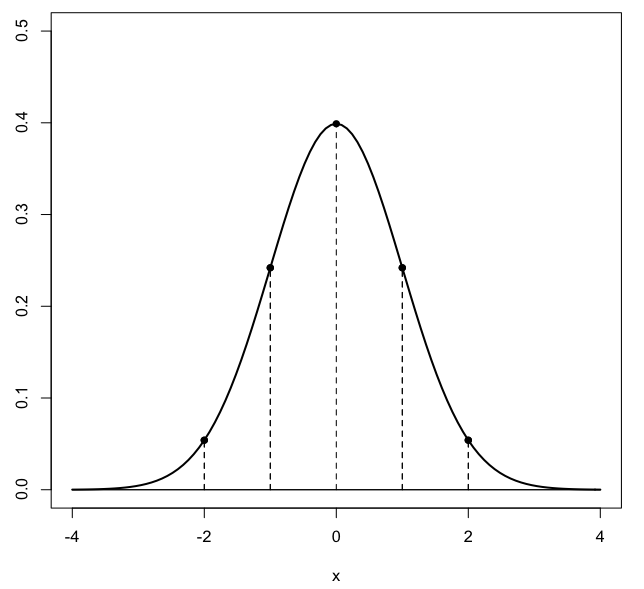
\includegraphics [scale=0.4] {gauss3.png} \end{center}
% \begin{bmatrix} a  &  b \\ c  &  d \end{bmatrix}
% \bigg |_

\begin{document}
\maketitle
\Large
%\noindent

Let's see if we can figure out the basic facts about surface integrals in the simplest possible way. 

For a point on a surface, we use the tangent plane approximation.  Imagine that the surface is tiled, composed of numerous tiny planes.  At any point, the surface is locally flat, having uniform slope and constant normal vector.  We will need to find the angle $\theta$ this plane makes with the horizontal.  We use that angle for this calculation:

\[ dA = \cos \theta \ dS \]
\[ dS = \frac{1}{\cos \theta} \ dA \]

A little piece of area on the surface is made smaller in its projection to the $xy$-plane by this factor.

Like any plane, we describe a tangent plane by its normal vector, $\mathbf{n}$.  You should be able to see that $\mathbf{n}$ makes the same angle $\theta$ with the $z$-axis or $\hat{\mathbf{k}}$ unit vector, so that

\[ \mathbf{n} \cdot \hat{\mathbf{k}} = |\mathbf{n}| |\hat{\mathbf{k}}| \ \cos \theta \]

Since $\hat{\mathbf{k}}$ is a unit vector, $|\hat{\mathbf{k}}| = 1$

\[ \mathbf{n} \cdot \hat{\mathbf{k}} = |\mathbf{n}| \ \cos \theta \]
\[ \frac{1}{\cos \theta} = \frac{\mathbf{n} \cdot \hat{\mathbf{k}} }{|\mathbf{n}|} \]

As always, we find $\mathbf{n}$ by first finding two vectors in the plane and then forming the cross-product.  We will use the basis vectors $( \hat{\mathbf{i}}, \hat{\mathbf{j}}, \hat{\mathbf{k}} )$, so we think about a cross-section of the plane at the point of interest, parallel to the $xz$-plane.  

The surface at the cross-section is just a line with some tilt to it, with slope $f_x$.  For each unit of change in $x$ or $\hat{\mathbf{i}}$ direction, there is a change of $f_x$ in the $\hat{\mathbf{k}}$ direction and none in the $\hat{\mathbf{j}}$ direction.  So one vector in the plane is

\[ \langle 1, 0, f_x \rangle \]

The second is, of course,

\[ \langle 0, 1, f_y \rangle \]

The cross-product is

\[ \langle -f_x, -f_y, 1 \rangle = \mathbf{n}  \]

We have formulated things so that $\mathbf{n} \cdot \hat{\mathbf{k}}$ is $1$!  Our currency exchange rate for area in the plane compared to area on the sloped tangent plane is 
just

\[ \frac{1}{\cos \theta} = \frac{\mathbf{n} \cdot \hat{\mathbf{k}}}{ |\mathbf{n}|} =  \frac{1}{|\mathbf{n}|} =  \frac{dS}{dA} \]
\[ dS = |\mathbf{n}| \ dA \]

and

\[ |\mathbf{n}| = \sqrt{1 + f_x^2 + f_y^2} \]

Hence 

\[ \iint_S \ dS = \iint \sqrt{1 + f_x^2 + f_y^2} \ dx \ dy \]

How about an example?  The hemisphere of radius $R$

\[ x^2 + y^2 + z^2 = R^2\]
\[ z = \sqrt{R^2 - x^2 - y^2} \]
\[ f_x = -\frac{x}{z} ; \ \ \ f_y = -\frac{y}{z} \]
\[ |\mathbf{n}| = \sqrt{1 + f_x^2 + f_y^2}  =  \sqrt{1 + (\frac{x}{z})^2 + (\frac{y}{z})^2} \]
\[ = \frac{1}{z}  \sqrt{z^2 + x^2 + y^2} = \frac{R}{z} \]

Hence

\[ SA = \iint |\mathbf{n}| \ dx \ dy = \iint \frac{R}{z} \ dx \ dy \]
\[ = R \iint \frac{1}{\sqrt{R^2-r^2}} \ r \ dr \ d \theta \]
\[ -2 \pi R\ [ \ \sqrt{R^2-r^2} \ ] \ \bigg |_0^R  = 2 \pi R^2  \]
and twice that for the sphere.
\end{document}  